\documentclass[aspectratio=169]{beamer}
\usetheme{Boadilla}
\usecolortheme{seahorse}
\usepackage[T1]{fontenc}
\usepackage{lmodern}
\usepackage{booktabs}
\usepackage{array}
\usepackage{amsmath}
\usepackage[table]{xcolor}
\usepackage{tikz}
\usetikzlibrary{arrows.meta,positioning,fit,backgrounds}

\setbeamertemplate{navigation symbols}{}
\setbeamertemplate{itemize items}[circle]
\setbeamerfont{frametitle}{size=\large}

%---------------------------------------------------------------- palette
\definecolor{ink}{HTML}{1F2933}
\definecolor{soft}{HTML}{6B7A8D}
\definecolor{hdr}{HTML}{3D5A73}
\definecolor{band}{HTML}{EDF2F7}
\definecolor{warm}{HTML}{C05621}
\definecolor{warmbg}{HTML}{FDF0E3}
\definecolor{cool}{HTML}{2C5282}
\definecolor{coolbg}{HTML}{E4EDF7}
\definecolor{good}{HTML}{2F6F4E}
% Bar-chart fill. A more chromatic sibling of `cool`: the frequency chart is the one
% place a fill carries meaning on its own, and `cool` is too desaturated to read as a
% colour there rather than as grey.
\definecolor{barA}{HTML}{2166BD}

%---------------------------------------------------------------- helpers
% A slide is 16:9 and short. Every box here is tuned so a full table plus a keybox
% still lands inside the frame -- vertical space is the scarce resource, not width.
\newcommand{\keybox}[1]{%
  \par\vspace{4pt}\begingroup\centering
  \colorbox{warmbg}{\parbox{0.93\textwidth}{\centering #1}}%
  \par\endgroup\vspace{2pt}}

\newcommand{\bigidea}[1]{%
  \vfill
  \begingroup\centering
  \colorbox{warmbg}{\parbox{0.93\textwidth}{\centering \large #1}}%
  \par\endgroup
  \vfill}

% Every table in this deck uses these lines: a coloured header, banded rows, no
% vertical rules, and \small rather than \scriptsize -- a table nobody can read is a
% table that is not in the talk.
\newenvironment{nicetable}[1]
  {\par\vspace{2pt}\begingroup\centering\small
   \renewcommand{\arraystretch}{1.18}%
   \setlength{\tabcolsep}{6pt}\rowcolors{2}{band}{white}%
   \begin{tabular}{#1}\arrayrulecolor{hdr}\toprule}
  {\bottomrule\end{tabular}\par\endgroup\vspace{2pt}}

% ---- the three blocks every worked example is made of ----------------
% One row of Madison's spreadsheet, drawn to look like a spreadsheet: header
% strip, one data row, same six columns every time so the shape is learnt once.
\newcommand{\sheetrow}[6]{%
  \par\vspace{3pt}\begingroup\centering\footnotesize
  \renewcommand{\arraystretch}{1.3}\setlength{\tabcolsep}{5pt}%
  \begin{tabular}{|>{\raggedright\arraybackslash}p{0.6cm}|>{\raggedright\arraybackslash}p{1.6cm}|>{\raggedright\arraybackslash}p{2.4cm}|>{\raggedright\arraybackslash}p{2.9cm}|>{\raggedright\arraybackslash}p{2.9cm}|>{\raggedright\arraybackslash}p{1.0cm}|}
  \hline
  \rowcolor{hdr}
  \textcolor{white}{\textbf{Line}} & \textcolor{white}{\textbf{Speaker}} &
  \textcolor{white}{\textbf{Error}} & \textcolor{white}{\textbf{AI Transcript}} &
  \textcolor{white}{\textbf{Actual Speech}} & \textcolor{white}{\textbf{Add Turn?}} \\
  \hline
  \rowcolor{warmbg}
  #1 & #2 & #3 & #4 & #5 & #6 \\
  \hline
  \end{tabular}\par\endgroup\vspace{4pt}}

% The machine's turns, and the turns after the fix.
\newcommand{\before}[1]{%
  \par\vspace{3pt}\begingroup\centering
  {\footnotesize\textcolor{soft}{\textbf{BEFORE}}}\par\vspace{1pt}
  \colorbox{coolbg}{\parbox{0.90\textwidth}{\ttfamily\footnotesize #1}}%
  \par\endgroup\vspace{3pt}}
\newcommand{\after}[1]{%
  \par\vspace{2pt}\begingroup\centering
  {\footnotesize\textcolor{good}{\textbf{AFTER}}}\par\vspace{1pt}
  \colorbox{band}{\parbox{0.90\textwidth}{\ttfamily\footnotesize #1}}%
  \par\endgroup\vspace{3pt}}

% The operation name, so the four verbs are visually identical everywhere.
\newcommand{\opn}[1]{\textcolor{warm}{\textbf{\texttt{#1}}}}

% ---- one row of the frequency chart -------------------------------------
% {row index, 0 at the top} {count} {label} {fill}. The enclosing tikzpicture sets
% x so that one unit is one row of the sheet, which is why the count is passed
% straight through as a width and again as its own printed label.
\newcommand{\barrow}[4]{%
  \fill[#4, rounded corners=1.2pt] (0,#1-0.28) rectangle (#2,#1+0.28);
  \node[ink, font=\small, anchor=east, xshift=-5pt] at (0,#1) {#3};
  \node[#4, font=\small\bfseries, anchor=west, xshift=4pt] at (#2,#1) {#2};}

% ---- the two sides of a computed grade ---------------------------------
% Deliberately NOT \before and \after. Those two mean "the machine's turns" and "the turns
% after the fix", and Part 5 is comparing the finished key against a DIFFERENT arm rather
% than showing one transcript being repaired. Same two colours, honest captions.
\newcommand{\keyblock}[1]{%
  \par\vspace{2pt}\begingroup\centering
  {\footnotesize\textcolor{good}{\textbf{THE ANSWER KEY}}}\par\vspace{1pt}
  \colorbox{band}{\parbox{0.92\textwidth}{\ttfamily\footnotesize #1}}%
  \par\endgroup\vspace{3pt}}
\newcommand{\armblock}[1]{%
  \par\vspace{2pt}\begingroup\centering
  {\footnotesize\textcolor{soft}{\textbf{WHAT THIS ARM PRODUCED}}}\par\vspace{1pt}
  \colorbox{coolbg}{\parbox{0.92\textwidth}{\ttfamily\footnotesize #1}}%
  \par\endgroup\vspace{3pt}}

% ---- one row of the two-cell comparison chart ---------------------------
% {row index} {count for the first cell} {count for the second} {label}. Two thin bars per
% row rather than one fat one, because the whole point of the slide is which labels have
% two DIFFERENT counts -- and a label whose two counts are equal has to read as one block
% at a glance, with no arithmetic.
\newcommand{\pairrow}[4]{%
  \fill[barA, rounded corners=1.0pt] (0,#1-0.30) rectangle (#2,#1-0.02);
  \fill[warm, rounded corners=1.0pt] (0,#1+0.02) rectangle (#3,#1+0.30);
  \node[ink, font=\small, anchor=east, xshift=-5pt] at (0,#1) {#4};
  \node[barA, font=\scriptsize\bfseries, anchor=west, xshift=3pt] at (#2,#1-0.16) {#2};
  \node[warm, font=\scriptsize\bfseries, anchor=west, xshift=3pt] at (#3,#1+0.16) {#3};}

% ---- one slab of the three-dimensional grid ----------------------------
% {x shift} {y shift} {cell fill} {cell border}. Four typists down, five name-taggers
% across, drawn as separated squares rather than a ruled table so the two slabs read as
% two sheets at different depths instead of as one table with too many lines.
\newcommand{\gridslab}[4]{%
  \begin{scope}[shift={(#1,#2)}]
    \foreach \r in {0,1,2,3}{\foreach \c in {0,1,2,3,4}{
      \fill[#3, draw=#4, line width=0.3pt, rounded corners=0.6pt]
        (\c,\r) rectangle (\c+0.74,\r+0.74);}}
  \end{scope}}

\newcommand{\hd}[1]{\textcolor{hdr}{\textbf{#1}}}
\newcommand{\typist}{\textbf{the typist}}
\newcommand{\timer}{\textbf{the stopwatch}}
\newcommand{\tagger}{\textbf{the name-tagger}}
\newcommand{\num}[1]{\textcolor{warm}{\textbf{#1}}}

\title{Did the Computer Hear It Right?}
\subtitle{The answer key, how we built it, and what we test next}
\author{PSYCH-ASR}
\date{}

\begin{document}

\frame{\titlepage}

%================================================================
\section{The picture}
\begin{frame}{Part 1 --- Three models and a piece of arithmetic}

Two robots work on the recording, and a third step glues their answers together.

\begin{nicetable}{ll}
\hd{Who} & \hd{What they do} \\ \midrule
\typist{}      & writes down every word that was said \\
\timer{}       & marks exactly when each word starts and stops \\
\tagger{}      & decides which of the two people was talking, and when \\
\end{nicetable}

\vspace{0.3em}
Put them together and you get \textbf{subtitles with names on them}:

\begin{center}
\small
\colorbox{band}{\parbox{0.62\textwidth}{\texttt{THERAPIST:~~So how was your week?}\\
\texttt{PATIENT:~~~~~It was okay I guess.}}}
\end{center}

\vspace{0.2em}
\keybox{\textbf{One line there is one ``turn''} --- a single unbroken stretch of one person
talking, ending when the other person starts. That box holds \textbf{two turns}. The whole
deck is about getting the turns right, so it is the one word worth keeping.}

\end{frame}

%----------------------------------------------------------
\begin{frame}{How the pieces fit together}

\begin{center}
\resizebox{0.95\textwidth}{!}{%
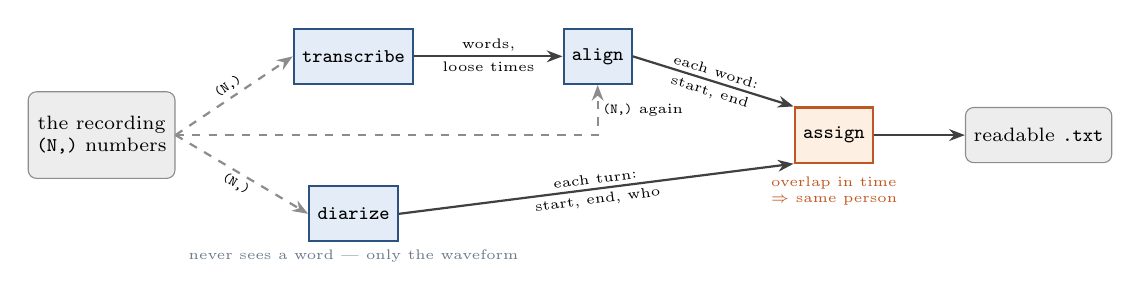
\begin{tikzpicture}[
  font=\scriptsize,
  >={Stealth[length=2mm]},
  data/.style={draw=black!45, rounded corners=3pt, fill=black!7,
               align=center, inner sep=3pt, minimum height=7mm},
  model/.style={draw=cool, thick, fill=coolbg,
                align=center, inner sep=3pt, minimum height=7mm},
  merge/.style={draw=warm, thick, fill=warmbg,
                align=center, inner sep=3pt, minimum height=7mm},
  flow/.style={->, thick, draw=black!75},
  bus/.style={->, thick, draw=black!45, dashed},
  lbl/.style={font=\tiny, inner sep=1.5pt}
]

\node[data, minimum height=11mm] (A) at (0,0) {the recording\\\texttt{(N,)} numbers};
\node[model] (T)  at (3.2,1.0)  {\texttt{transcribe}};
\node[model] (AL) at (6.3,1.0)  {\texttt{align}};
\node[model] (D)  at (3.2,-1.0) {\texttt{diarize}};
\node[merge] (AS) at (9.3,0)    {\texttt{assign}};
\node[data]  (R)  at (11.9,0)   {readable \texttt{.txt}};

\draw[bus] (A.east) -- node[lbl, above, sloped] {\texttt{(N,)}} (T.west);
\draw[bus] (A.east) -- node[lbl, below, sloped] {\texttt{(N,)}} (D.west);
\draw[bus] (A.east) -- (6.3,0) -- node[lbl, right] {\texttt{(N,)} again} (AL.south);

\draw[flow] (T) -- node[lbl, above] {words,}
                   node[lbl, below] {loose times} (AL);
\draw[flow] (AL.east) -- node[lbl, above, sloped] {each word:}
                         node[lbl, below, sloped] {start, end} (AS.north west);
\draw[flow] (D.east) -- node[lbl, above, sloped] {each turn:}
                        node[lbl, below, sloped] {start, end, who} (AS.south west);
\draw[flow] (AS) -- (R);

\node[lbl, text=soft, below=1pt of D] {never sees a word --- only the waveform};
\node[lbl, text=warm, below=3pt of AS, align=center]
      {overlap in time\\$\Rightarrow$ same person};
\end{tikzpicture}}
\end{center}

\keybox{Three boxes do real work: \texttt{transcribe} is \typist{}, \texttt{align} is
\timer{}, \texttt{diarize} is \tagger{}. \texttt{assign} is not a model --- it is
arithmetic on the two lists of times.}

\end{frame}

%----------------------------------------------------------
\begin{frame}{Three of those boxes are choices}

\texttt{assign} is arithmetic and has no alternatives. The other three are \textbf{models we
picked}, and every one of them can be swapped for a different model.

\begin{center}
\resizebox{0.92\textwidth}{!}{%
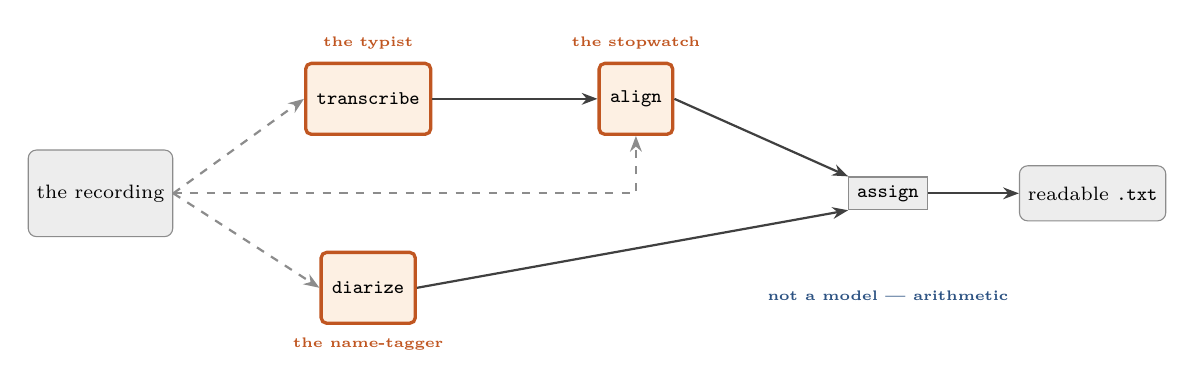
\begin{tikzpicture}[
  font=\scriptsize,
  >={Stealth[length=2mm]},
  data/.style={draw=black!45, rounded corners=3pt, fill=black!7,
               align=center, inner sep=3pt, minimum height=7mm},
  swap/.style={draw=warm, very thick, fill=warmbg, rounded corners=2pt,
               align=center, inner sep=4pt, minimum height=9mm},
  merge/.style={draw=black!45, fill=black!7, align=center, inner sep=3pt},
  flow/.style={->, thick, draw=black!75},
  bus/.style={->, thick, draw=black!45, dashed},
  lbl/.style={font=\tiny, inner sep=1.5pt},
  tag/.style={font=\tiny\bfseries, text=warm}
]

\node[data, minimum height=11mm] (A) at (0,0) {the recording};
\node[swap] (T)  at (3.4,1.2)  {\texttt{transcribe}};
\node[swap] (AL) at (6.8,1.2)  {\texttt{align}};
\node[swap] (D)  at (3.4,-1.2) {\texttt{diarize}};
\node[merge] (AS) at (10.0,0)  {\texttt{assign}};
\node[data]  (R)  at (12.6,0)  {readable \texttt{.txt}};

\node[tag, above=1pt of T]  {the typist};
\node[tag, above=1pt of AL] {the stopwatch};
\node[tag, below=1pt of D]  {the name-tagger};

\draw[bus] (A.east) -- (T.west);
\draw[bus] (A.east) -- (D.west);
\draw[bus] (A.east) -- (6.8,0) -- (AL.south);
\draw[flow] (T) -- (AL);
\draw[flow] (AL.east) -- (AS.north west);
\draw[flow] (D.east) -- (AS.south west);
\draw[flow] (AS) -- (R);

\node[tag, text=cool] at (10.0,-1.3) {not a model --- arithmetic};
\end{tikzpicture}}
\end{center}

\bigidea{Wrong words, wrong times, or wrong names. Three separate failures, three separate
models to test.}

\end{frame}

%================================================================
\section{Madison's spreadsheet}
\begin{frame}{Part 2 --- The answer key}

To say one model beats another you need to know what the \emph{right} answer was. That is
what Madison built.

\vspace{0.5em}
She opened the machine's transcript as a plain text file with \textbf{numbered lines}, put
the audio on, and listened to the whole session. Every time the machine got something wrong,
she added \textbf{one row} to a spreadsheet.

\vspace{0.5em}
She is not writing a transcript from scratch. She is recording the \emph{difference} between
what the machine said and what she heard.

\bigidea{117 rows. Fifty minutes of listening.\\[3pt]
That spreadsheet is the entire ground truth this project has.}

\end{frame}

%----------------------------------------------------------
\begin{frame}{What is in one row}

\begin{nicetable}{p{2.9cm}p{9.6cm}}
\hd{Column} & \hd{What it holds} \\ \midrule
Timestamp     & where she heard it \\
Line          & the line number in the machine's text file --- her only pointer into the machine's own version \\
Speaker       & who \emph{really} said it: Therapist or Participant \\
Error         & one of six labels (next slide) \\
AI Transcript & what the machine wrote there --- or the word \texttt{None} if it wrote nothing \\
Actual Speech & what was really said --- or \texttt{None} if nothing was \\
Severity      & her judgement of how much it matters \\
\textbf{Add Turn?} & \textbf{TRUE if fixing this creates a turn the machine never produced} \\
\end{nicetable}

\keybox{Two columns carry the weight. \textbf{Line} says \emph{where}; \textbf{Add Turn?}
says whether the \emph{words} or the \emph{conversation's shape} went wrong.}

\end{frame}

%----------------------------------------------------------
\begin{frame}{The six kinds of error}

\begin{nicetable}{p{3.3cm}p{9.2cm}}
\hd{Label} & \hd{What went wrong} \\ \midrule
Omission            & something was said and the machine wrote nothing \\
Insertion           & the machine wrote something nobody said \\
Substitution        & the machine wrote the wrong words \\
Proper Noun         & a name or place came out mangled \\
Punctuation         & the words are right, the sentence breaks are not \\
\textbf{Speaker Attribution} & \textbf{the words are right and they are filed under the wrong person} \\
\end{nicetable}

\vspace{0.3em}
The first five are \typist{} making mistakes. The last one is \tagger{} making mistakes ---
the machine heard perfectly and pointed at the wrong person.

\keybox{\num{32} of the 117 rows are Speaker Attribution. Those are the rows that grade
the part of the pipeline the whole project depends on.}

\end{frame}

%----------------------------------------------------------
% Frequency of the six labels. Counts are the by_error tally from the Stage 2
% correction pass (applied + already-done + superseded + unplaced, so every row is
% counted exactly once): 69 + 32 + 9 + 5 + 1 + 1 = 117.
\begin{frame}{How often each kind happened}

Six labels, 117 rows --- and two of the labels are almost the whole sheet.

\vspace{0.2em}
\begin{center}
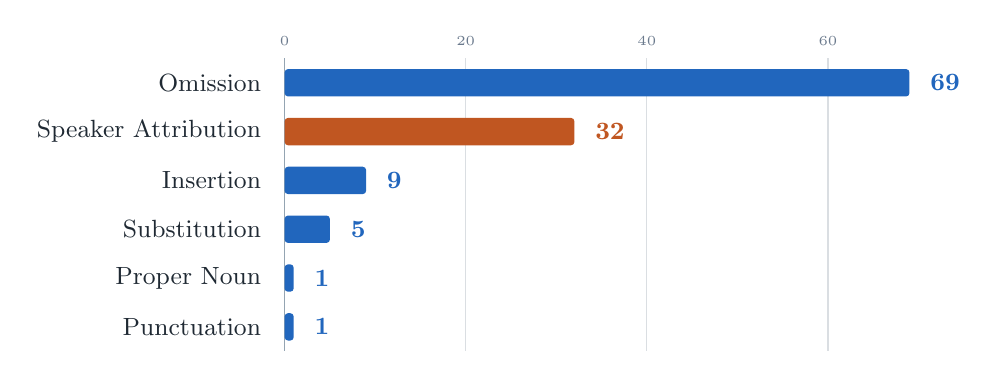
\begin{tikzpicture}[x=0.115cm, y=-0.62cm]
  % scale, along the top: recessive, four ticks, no box
  \foreach \g in {0,20,40,60}{
    \draw[soft!25, line width=0.4pt] (\g,-0.5) -- (\g,5.5);
    \node[soft, font=\tiny, anchor=south, yshift=1pt] at (\g,-0.5) {\g};}
  \draw[hdr!55, line width=0.6pt] (0,-0.5) -- (0,5.5);

  \barrow{0}{69}{Omission}{barA}
  \barrow{1}{32}{Speaker Attribution}{warm}
  \barrow{2}{9}{Insertion}{barA}
  \barrow{3}{5}{Substitution}{barA}
  \barrow{4}{1}{Proper Noun}{barA}
  \barrow{5}{1}{Punctuation}{barA}
\end{tikzpicture}
\end{center}

\vspace{-0.2em}
{\footnotesize
\tikz[baseline=-0.55ex]\fill[barA, rounded corners=1pt] (0,0) rectangle (7pt,7pt);\,
\textcolor{soft}{\typist{} mis-hearing}\qquad
\tikz[baseline=-0.55ex]\fill[warm, rounded corners=1pt] (0,0) rectangle (7pt,7pt);\,
\textcolor{soft}{\tagger{} mis-filing}}

\keybox{\num{69} omissions and \num{32} misattributions are \num{101} of the 117 rows.
Punctuation and mangled names happen \textbf{once each}.}

\end{frame}

%----------------------------------------------------------
% The three shapes, on invented lines rather than session content, and BEFORE the table
% that counts them -- the table's rows are unreadable until the reader knows what "add or
% move a turn" means. The first two examples deliberately share the same right-hand
% column: what was really said is identical, and only the machine's version differs. That
% IS the difference between adding a turn and moving one.
\begin{frame}{Three ways the machine can be wrong}

Every one of the 117 rows is one of these three shapes. Invented exchanges;
\texttt{T} is the therapist, \texttt{P} the participant.

\begin{nicetable}{p{1.9cm}p{4.9cm}p{4.0cm}}
\hd{} & \hd{What the machine produced} & \hd{What was really said} \\ \midrule
\hd{Turn added}
  & \ttfamily T~~did it help
  & \ttfamily T~~did it help\newline \textbf{P~~not really} \\
\hd{Turn moved}
  & \ttfamily T~~did it help not really
  & \ttfamily T~~did it help\newline \textbf{P~~not really} \\
\hd{Words only}
  & \ttfamily P~~it was tuesday
  & \ttfamily P~~it was \textbf{thursday} \\
\end{nicetable}

\vspace{0.1em}
{\small \textbf{The first two want the same answer.} ``Not really'' is the participant's
own turn either way. They differ only in what the machine did with it: in the first it never
wrote those words at all, in the second it wrote them inside the therapist's turn. Both
fixes end with \num{one more turn} on the page than the machine produced.}

\keybox{Only the third leaves the turns alone. The first two change \textbf{who spoke, and
when} --- and that is what every structural feature we plan to measure is counted from.}

\end{frame}

%----------------------------------------------------------
\begin{frame}{Most of the sheet is about turns, not spelling}

One column, \textbf{Add Turn?}, is ticked when fixing the row would \emph{add or move a
turn} --- the first two shapes --- rather than just change the words inside one. Split the
117 rows on that tick:

\begin{nicetable}{p{8.2cm}r}
\hd{What the machine did} & \hd{Rows} \\ \midrule
Missed something a person said, completely      & 47 \\
Put one person's words inside the other's turn  & 27 \\
Wrote down something nobody said                & 1 \\ \midrule
\rowcolor{warmbg} \textbf{Turns wrong} --- ticked & \num{75} \\
Wrote the wrong words; the turns were right     & 42 \\ \midrule
\rowcolor{band} \textbf{Every row in the sheet} & \textbf{117} \\
\end{nicetable}

\keybox{\num{75} of the 117 rows are \emph{turn added} or \emph{turn moved}. Only the
\num{42} are \emph{words only}.}

\end{frame}
%================================================================
\section{Rebuilding the transcript}
\begin{frame}{Part 3 --- One row, one fix}

Every one of the 117 rows becomes exactly one edit. The next six slides are the whole
algorithm: \textbf{her row, the machine's turns before, the turns after.}

\vspace{0.6em}
There are only four things the program can do, and \textbf{Add Turn?} is what picks between
them:

\begin{nicetable}{p{2.3cm}p{7.0cm}r}
\hd{Operation} & \hd{What changes} & \hd{Used} \\ \midrule
\textbf{replace} & the words inside one turn & 35 \\
\textbf{insert}  & a new turn appears & 53 \\
\textbf{extract} & words move out into a turn of their own & 21 \\
\textbf{relabel} & the name on a turn & 5 \\
\end{nicetable}

\keybox{Only \textbf{replace} leaves the turns alone. The other three are why this is not
find-and-replace.}

\end{frame}

%----------------------------------------------------------
\begin{frame}{Example 1 --- the machine misheard a word}

\sheetrow{132}{Participant}{Substitution}{really tired lately}{really wired lately}{FALSE}

\before{PARTICIPANT~~[12:04--12:09]~~i've been really tired lately}

\after{PARTICIPANT~~[12:04--12:09]~~i've been really wired lately}

\keybox{\opn{replace}. One turn in, one turn out. Same speaker, same times, three
characters different. \textbf{Proper Noun} and \textbf{Punctuation} rows do exactly this
too --- a mangled name, a sentence broken in the wrong place.}

\end{frame}

%----------------------------------------------------------
\begin{frame}{Example 2 --- words dropped out of the middle of a turn}

\sheetrow{88}{Therapist}{Omission}{\textit{None}}{for the whole week}{FALSE}

{\footnotesize \textit{None} leaves no words to search for, so \texttt{Line 88} is the
only anchor --- and it names a \emph{line} of the file, not a turn. Her own numbered view:}

\before{~~87~~[08:15]~THERAPIST\\
~~88~~~~so~you~did~that~every~day\\
\textcolor{warm}{~~~~~~~~~~~~~~~~~~~~~~~~~~~~~~~~~\textasciicircum{}~the~end~of~line~88's~words}}

\after{~~87~~[08:15]~THERAPIST\\
~~88~~~~so~you~did~that~every~day~\textbf{for~the~whole~week}}

\keybox{\opn{replace} at a single point: \textbf{the end of line 88's words}. Nothing in the
sheet says where inside the line they go --- that is assumed, and it is the one thing this
row cannot pin down. \textbf{Add Turn? is FALSE}, so the shape of the conversation is
unchanged.}

\end{frame}

%----------------------------------------------------------
\begin{frame}{Example 3 --- something somebody said, missed completely}

\sheetrow{205}{Participant}{Omission}{\textit{None}}{mm hmm}{\textbf{TRUE}}

\before{THERAPIST~~~~[19:40--19:58]~~and that's the part we want to build on next week}

\after{THERAPIST~~~~[19:40--19:51]~~and that's the part we want to build on\\
PARTICIPANT~~[19:51--19:51]~~mm hmm\\
THERAPIST~~~~[19:51--19:58]~~next week}

\keybox{\opn{insert}. Now \textbf{Add Turn? is TRUE}, so a turn that never existed appears
--- and the therapist's turn is cut in two around it. \textbf{One turn became three.} There
were \num{47} rows like this.}

\end{frame}

%----------------------------------------------------------
\begin{frame}{Example 4 --- two people welded into one turn}

\sheetrow{48}{Participant}{Speaker Attribution}{yeah \textbf{Therapist}}{yeah \textbf{Participant}}{\textbf{TRUE}}

\before{THERAPIST~~~~[04:12--04:31]~~did you try the walk yeah so how did that go}

\after{THERAPIST~~~~[04:12--04:20]~~did you try the walk\\
PARTICIPANT~~[04:20--04:22]~~yeah\\
THERAPIST~~~~[04:22--04:31]~~so how did that go}

\keybox{\opn{extract}. The words were transcribed perfectly --- they were filed under the
wrong person. \textbf{Look at the two text cells: both end in a role name.} That is her
convention, and it is how the program knows the machine said ``Therapist'' where the truth
was ``Participant''.}

\end{frame}

%----------------------------------------------------------
\begin{frame}{Example 5 --- the right words under the wrong name}

\sheetrow{301}{Therapist}{Speaker Attribution}{how did that feel \textbf{Participant}}{how did that feel \textbf{Therapist}}{FALSE}

\before{PARTICIPANT~~[28:03--28:07]~~and how did that feel}

\after{THERAPIST~~~~[28:03--28:07]~~and how did that feel}

\keybox{\opn{relabel}. Same words, same times, one name changed. \textbf{Add Turn? is
FALSE} because the machine did find a turn here --- it just put the wrong person's name on
the front of it. Only \num{5} rows are this simple.}

\end{frame}

%----------------------------------------------------------
\begin{frame}{Example 6 --- the machine wrote something nobody said}

\sheetrow{156}{Participant}{Insertion}{thank you for watching}{\textit{None}}{FALSE}

\before{PARTICIPANT~~[14:22--14:30]~~i guess so thank you for watching}

\after{PARTICIPANT~~[14:22--14:30]~~i guess so}

\keybox{\opn{replace}, with nothing. This one is worth recognising: ``thank you for
watching'' is a phrase \typist{} learnt from video subtitles and emits into \textbf{silence}.
It is not a mishearing --- there was no sound there at all.}

\end{frame}

%----------------------------------------------------------
\begin{frame}{The case that needs care --- two rows, one ``yeah''}

Madison logs a misattribution \textbf{twice}, from both sides:

\sheetrow{48}{Participant}{Speaker Attribution}{yeah \textbf{Therapist}}{yeah \textbf{Participant}}{\textbf{TRUE}}
\vspace{-6pt}
\sheetrow{49}{Therapist}{Insertion}{yeah}{\textit{None}}{FALSE}

\vspace{0.3em}
Row 48 says \emph{move that ``yeah'' to the participant}. Row 49 says \emph{take that
``yeah'' out of the therapist's turn}. \textbf{They describe the same three characters} ---
and moving them \emph{is} taking them out.

\keybox{Run both and the word is deleted twice. So the first edit \textbf{claims} those
characters, and row 49 is reported as \emph{already handled} --- not applied, and not a
failure either. One row on this sheet ended up in that pile.}

\end{frame}

%----------------------------------------------------------
\begin{frame}{The result}

\begin{nicetable}{p{5.0cm}rr}
\hd{} & \hd{Machine} & \hd{Corrected} \\ \midrule
Turns          & 89      & \num{215} \\
Words          & 7{,}298 & 7{,}388 \\
Speaker labels & anonymous & Therapist / Participant \\
\end{nicetable}

\vspace{0.2em}
Of the 117 rows: \num{114} applied, 1 already handled by an earlier row, and 2 the program
refused to place --- it could not find her words, so it \textbf{changed nothing} and named
the rows.

\bigidea{The machine heard \num{89} back-and-forths. There were \num{215}.\\[3pt]
It loses the short ones --- and the short ones are most of the conversation's shape.}

\end{frame}

%----------------------------------------------------------
\begin{frame}{The sheet also names the speakers, for free}

Look at Example 4's row again. The \textbf{AI Transcript} cell says what the machine
decided:

\sheetrow{48}{Participant}{Speaker Attribution}{yeah \textbf{Therapist}}{yeah \textbf{Participant}}{\textbf{TRUE}}

\vspace{0.3em}
The machine's own label for that turn is \texttt{SPEAKER\_00}. Madison wrote that the machine
called it \emph{Therapist}. So \texttt{SPEAKER\_00} \textbf{is} the therapist --- stated, not
guessed. Across the sheet: \num{49} rows say so, 3 disagree.

\keybox{And it \textbf{inverts} the obvious guess. In the corrected transcript the therapist
holds \num{78.6\%} of the talk time --- session 1 is the didactic intro. ``The therapist
talks less'' would have got this session exactly backwards.}

\end{frame}

%----------------------------------------------------------
\begin{frame}{What this reference cannot do --- look at Example 3 again}

\after{THERAPIST~~~~[19:40--19:51]~~and that's the part we want to build on\\
PARTICIPANT~~[19:51--19:51]~~mm hmm\\
THERAPIST~~~~[19:51--19:58]~~next week}

\vspace{0.1em}
\textbf{That ``mm hmm'' lasts zero seconds}, and 19:51 is a guess --- the split fell where
the \emph{characters} divide, not the sound.

\begin{nicetable}{p{6.0cm}p{6.4cm}}
\hd{So it can grade} & \hd{It cannot grade} \\ \midrule
Were the words right? & Were the times right? \\
Was the speaker right? & Where exactly a turn starts and stops \\
Did the machine find the turn at all? & Anything measured in seconds \\
 & \textbf{Where inside a turn a word belongs} \\
\end{nicetable}

\keybox{Fixing the \emph{times} is one job: run \timer{} over the audio using Madison's
corrected words as the script. Then every word has a measured time.}

\end{frame}

%----------------------------------------------------------
% The within-line placement limit, on invented lines. This is the one cost of the Line
% column that the timing slide does not cover: 58 of the 117 rows are placed by line
% number alone, and a line number cannot say WHERE INSIDE the line the words go.
\begin{frame}{\ldots and it cannot place words inside a line}

\textbf{Line} names one \emph{wrapped} line of the file, not a whole turn. A long turn is
several numbered lines:

\begin{center}
\colorbox{band}{\parbox{0.86\textwidth}{\ttfamily\footnotesize
~~~~~~~~[12:30]~PARTICIPANT\\
~~~41~~~~i~went~for~a~walk~and~felt~better\\
~~~42~~~~so~i~tried~it~again~on~sunday}}
\end{center}
{\footnotesize\textcolor{soft}{Invented lines, narrowed to fit the slide; the real file
wraps at 96 characters.}}

\vspace{0.3em}
Madison logs \texttt{Line 41}, \textbf{Omission}, \textit{None}, ``with my dog''. Those
words were really said just after ``walk'' --- in the \emph{middle} of line 41. But
\textit{None} leaves nothing to search for, so the only anchor is the line:

\begin{nicetable}{p{3.2cm}p{8.3cm}}
\textcolor{good}{\textbf{Where they belong}}
  & \ttfamily i~went~for~a~walk~\textcolor{good}{\textbf{with~my~dog}}~and~felt~better \\
\textcolor{warm}{\textbf{Where they land}}
  & \ttfamily i~went~for~a~walk~and~felt~better~\textcolor{warm}{\textbf{with~my~dog}} \\
\end{nicetable}

\keybox{Same turn, same speaker, same words --- only the \emph{position} is wrong. That
costs the diarizer score nothing and the reference text a little. \num{58} of the 117 rows
are placed by line number alone.}

\end{frame}

%================================================================
\section{What we test next}
\begin{frame}{Part 4 --- Three models, and only one has been compared}

\begin{nicetable}{p{2.6cm}p{2.6cm}p{4.2cm}p{2.4cm}}
\hd{Box} & \hd{Nickname} & \hd{What runs today} & \hd{Compared?} \\ \midrule
\texttt{transcribe} & the typist & Whisper large-v3 & \textcolor{warm}{\textbf{no}} \\
\texttt{align} & the stopwatch & wav2vec2 base, trained on read audiobooks & \textcolor{warm}{\textbf{no}} \\
\texttt{diarize} & the name-tagger & five candidates & yes --- undecided \\
\end{nicetable}

\vspace{0.3em}
The stopwatch is the uncomfortable one: it is the \emph{small} model, trained on 960 hours of
people \textbf{reading books aloud}. Therapy speech is spontaneous, overlapped and disfluent.

\bigidea{Now that there is an answer key, all three can finally be graded.}

\end{frame}

%----------------------------------------------------------
% THE GRID IS A CUBE, NOT A TABLE, and the previous slide is what makes that unavoidable:
% it lists THREE swappable boxes. An earlier version of this slide swept two of them and
% left the stopwatch out of the very grid that exists because nobody had noticed it was a
% variable. Two slabs rather than a perspective box, because five columns of cell labels
% only fit on a face the reader is looking at straight on.
\begin{frame}{The grid has three axes, not two}

Three boxes are swappable, so the sweep is a \textbf{cube}: \num{4} typists $\times$
\num{2} stopwatches $\times$ \num{5} name-taggers $=$ \num{40} cells.

\vspace{0.1em}
\begin{center}
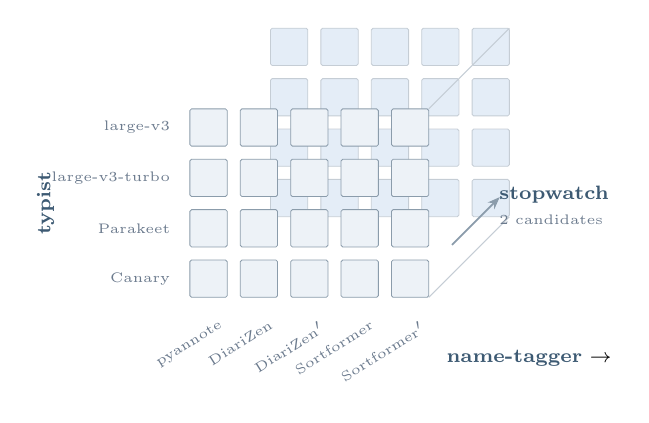
\begin{tikzpicture}[x=0.64cm, y=-0.64cm]
  % The far slab first, up and to the right, so the near one overlaps it and the pair reads
  % as depth rather than as two unrelated tables.
  \gridslab{1.6}{-1.6}{coolbg}{hdr!30}
  \gridslab{0}{0}{band}{hdr!60}
  % Depth guides off BOTH right-hand corners of the near slab: one line is an accident, two
  % parallel ones are a box.
  \draw[hdr!30, line width=0.4pt] (4.74,0) -- (6.34,-1.6);
  \draw[hdr!30, line width=0.4pt] (4.74,3.74) -- (6.34,2.14);
  \draw[hdr!60, line width=0.6pt, -{Stealth[length=4.5pt]}] (5.2,2.7) -- (6.15,1.75);
  \node[anchor=west, font=\scriptsize] at (5.95,1.7) {\hd{stopwatch}};
  \node[soft, font=\tiny, anchor=west] at (5.95,2.2) {2 candidates};
  % The typist axis, down the left of the near slab. No arrow on the rotated label: the
  % y axis is flipped here, so a down-arrow inside a 90-degree rotation points up.
  \node[rotate=90, anchor=south, font=\scriptsize] at (-2.5,1.87) {\hd{typist}};
  \foreach \r/\name in {0/large-v3, 1/large-v3-turbo, 2/Parakeet, 3/Canary}{
    \node[soft, font=\tiny, anchor=east] at (-0.2,\r+0.37) {\name};}
  % The name-tagger axis, along the bottom. Rotated because five model names do not fit
  % across five columns, and shrinking them to fit is how a figure stops being read.
  \foreach \c/\name in {0/pyannote, 1/DiariZen, 2/DiariZen$'$,
                        3/Sortformer, 4/Sortformer$'$}{
    \node[soft, font=\tiny, anchor=north east, rotate=32] at (\c+0.62,3.92) {\name};}
  \node[anchor=west, font=\scriptsize] at (4.9,4.95) {\hd{name-tagger} $\rightarrow$};
\end{tikzpicture}
\end{center}

\keybox{\textbf{Still cheaper than it looks.} \tagger{} never reads a word, so its answer
depends on neither of the other two. \num{4}$\times$\num{2} runs that write the words and
time them, plus \num{5} that only listen --- \textbf{13 jobs, not 40} --- and the cells are
assembled from the pieces.}

\end{frame}

%----------------------------------------------------------
% WHY THE CUBE IS NOT 40 INDEPENDENT MEASUREMENTS. This slide is the reason the grading
% algorithm two slides later is affordable: five of its six labels are a property of the
% typist alone, so a whole row of the grid shares them.
\begin{frame}{Each axis can only move some of the numbers}

The words come from the typist. The times come from the stopwatch, timing the typist's
words. Who-spoke comes from the name-tagger, which never reads a word.

\begin{nicetable}{p{2.8cm}p{1.9cm}p{1.9cm}p{4.7cm}}
\hd{Swap this} & \hd{Words change?} & \hd{Times change?} & \hd{So it can move} \\ \midrule
\typist{}   & \textcolor{warm}{\textbf{yes}} & \textcolor{warm}{\textbf{yes}}
            & every kind of error \\
\timer{}    & no & \textcolor{warm}{\textbf{yes}}
            & who-spoke only --- the times are what hand each word to a speaker \\
\tagger{}   & no & no
            & who-spoke only \\
\end{nicetable}

\keybox{Fix the typist and \textbf{five of the six error counts are already decided} for
that whole row of the grid --- one measurement per row plus one per cell, not six per cell.
The \emph{counts}, not their turn-or-words split: whether a missing utterance was a whole
turn depends on where the name-tagger put its boundaries.}

\end{frame}

%================================================================
\section{Grading the rest}
% PART 5. The reason this part exists at all: the answer key was built by a person, and a
% person cannot be asked to do it forty times.
\begin{frame}{Part 5 --- 39 more cells, and nobody is going to listen to them}

Madison's pass produced \textbf{one} cell of that cube. It cost fifty minutes of listening
and 117 typed rows.

\begin{nicetable}{p{5.6cm}p{6.6cm}}
\hd{What she did, once} & \hd{What we need, 39 more times} \\ \midrule
Listened to the recording & \textcolor{warm}{nobody has fifty minutes $\times$ 39} \\
Compared it to the machine's words & Compare it to \emph{her corrected transcript} instead \\
Wrote down each error and its kind & Count the same kinds, the same way \\
\end{nicetable}

\vspace{0.2em}
The corrected transcript is the recording's stand-in. Every question she answered by
listening --- was this word right, was this the right person, did the machine even find
this turn --- can be answered by comparing two pieces of text.

\bigidea{Grade against the answer key, not against the audio.\\[3pt]
Fifty minutes becomes two seconds, and it runs on a laptop.}

\end{frame}

%----------------------------------------------------------
\begin{frame}{The whole algorithm, in three steps}

\begin{nicetable}{p{0.5cm}p{4.0cm}p{7.6cm}}
\hd{} & \hd{Step} & \hd{Why it is in this order} \\ \midrule
1 & Line the two word lists up, \textbf{ignoring who spoke}
  & Which words match is the one question that must not be influenced by the speaker
    labels, or the grade starts assuming its own answer \\
2 & Read off \textbf{which cluster is whom}, from the words that matched
  & \texttt{SPEAKER\_00} is nobody until its words agree with the key's. A word both sides
    wrote is the only place the two naming schemes can be compared \\
3 & Ask \textbf{two questions} of every word
  & \emph{was it written down, and as itself} --- then, of the words that were,
    \emph{is it under the right person} \\
\end{nicetable}

\vspace{0.1em}
{\small Step 3 is why this is not just a word error rate. A single percentage cannot tell
an arm that mistyped forty words apart from an arm that filed forty \emph{correct} words
under the wrong person --- and those break different things downstream.}

\keybox{No timestamp is ever read. The key's turn times are interpolated guesses
(slide 21), so a grade that used them would be grading the guess. \textbf{Words and names
only}, which is exactly the part of the key that is trustworthy.}

\end{frame}

%----------------------------------------------------------
% THE WORKED EXAMPLE, and it is real output: these four findings are what the grader
% actually emitted on this invented pair of transcripts, not a hand-drawn illustration of
% what it might emit. Invented lines throughout -- no session content.
\begin{frame}{One session, one arm, four differences}

Invented lines. \texttt{T} is the therapist, \texttt{P} the participant; the arm's own
speaker names are still numbers, because that is all a name-tagger ever produces.

\keyblock{T~[00:00--00:06]~~so~how~was~your~week~and~did~the~activity~schedule~help~at~all\\
P~[00:06--00:06]~~\textbf{mm~hmm}\\
P~[00:06--00:12]~~\textbf{it~was~fine}~i~went~for~a~walk~with~my~dog~on~\textbf{thursday}\\
T~[00:12--00:16]~~tell~me~more~about~\textbf{Madison}~and~what~she~said}

\armblock{SPEAKER\_00~~so~how~was~your~week~and~did~the~activity~schedule~help~at~all~\textbf{it~was~fine}\\
SPEAKER\_01~~i~went~for~a~walk~with~my~dog~on~\textbf{tuesday}\\
SPEAKER\_00~~tell~me~more~about~\textbf{Madeline}~and~what~she~said}

\keybox{\textbf{Four things are wrong, and only two of them are spelling.} The arm lost
\texttt{mm~hmm} entirely, and it filed \texttt{it~was~fine} --- which it transcribed
\emph{perfectly} --- inside the therapist's turn.}

\end{frame}

%----------------------------------------------------------
% The four findings this pass actually emitted on the pair above -- real grader output on
% invented text, not a hand-drawn illustration of what it might have said.
\begin{frame}{What the grader called them}

\begin{nicetable}{p{2.5cm}p{1.8cm}p{1.8cm}p{1.2cm}p{4.1cm}}
\hd{Label} & \hd{Key says} & \hd{Arm said} & \hd{Turns wrong?} & \hd{Found by} \\
\midrule
Omission & \ttfamily mm hmm & \ttfamily --- & \textcolor{warm}{\textbf{yes}}
  & key words with nothing opposite \\
Speaker Attribution & \ttfamily it was fine & \ttfamily it was fine
  & \textcolor{warm}{\textbf{yes}}
  & words matched, the \emph{name} did not \\
Substitution & \ttfamily thursday & \ttfamily tuesday & no
  & one word standing for another \\
Proper Noun & \ttfamily Madison & \ttfamily Madeline & no
  & same, but capitalized \emph{mid-sentence} \\
\end{nicetable}

\keybox{\num{5} of the \num{6} labels fall out of lining the words up. The sixth ---
\emph{Speaker Attribution} --- is found among the words that \textbf{matched}, which is why
a grade that stopped at the word error rate would call this transcript good.}

\end{frame}

%----------------------------------------------------------
% THE ONE JUDGEMENT IN THE ALGORITHM. Everything else is mechanical; this is the rule that
% reproduces her Add Turn? column, and it is worth its own slide because a wrong answer
% here moves a row between the 75 and the 42.
\begin{frame}{The only judgement: did the turns change?}

Her \textbf{Add Turn?} column is not in the text --- it is a question about the text. One
rule answers it, and it is the same rule in both directions:

\bigidea{Is the \emph{whole} turn involved, or only part of one?}

\begin{nicetable}{p{3.2cm}p{4.6cm}p{4.4cm}}
\hd{} & \hd{Every word of the turn} & \hd{Only some of its words} \\ \midrule
\hd{Words missing} & the machine never heard this turn ---
  \textcolor{warm}{\textbf{a turn appears}}
  & it heard the turn and mistyped it --- \textbf{words only} \\
\hd{Wrong speaker} & the boundary is right, the name is wrong --- \textbf{words only}
  & fixing it \textcolor{warm}{\textbf{cuts the machine's turn open}} \\
\hd{Words invented} & \textcolor{warm}{\textbf{a turn disappears}} & \textbf{words only} \\
\end{nicetable}

\keybox{In the example: \texttt{mm hmm} is the participant's whole turn, so a turn appears.
\texttt{it was fine} is only part of the machine's first turn, so that turn gets cut open.
\num{2} of the \num{4} findings change the turn structure --- her ratio, computed.}

\end{frame}

%----------------------------------------------------------
% THE PAYOFF SLIDE: slide 8's chart, once per cell. The numbers are INVENTED and the slide
% says so twice, because the deck's own rule is that nothing is presented as measured until
% it is. What is NOT invented is the shape: five bars identical and one moving is a
% consequence of the pipeline, stated on the "each axis" slide and visible here.
\begin{frame}{What comes out: slide 8's chart, once per cell}

Same typist and stopwatch, two different name-taggers.
\textcolor{warm}{\textbf{Invented numbers}} --- no cell has been measured.

\vspace{0.1em}
\begin{center}
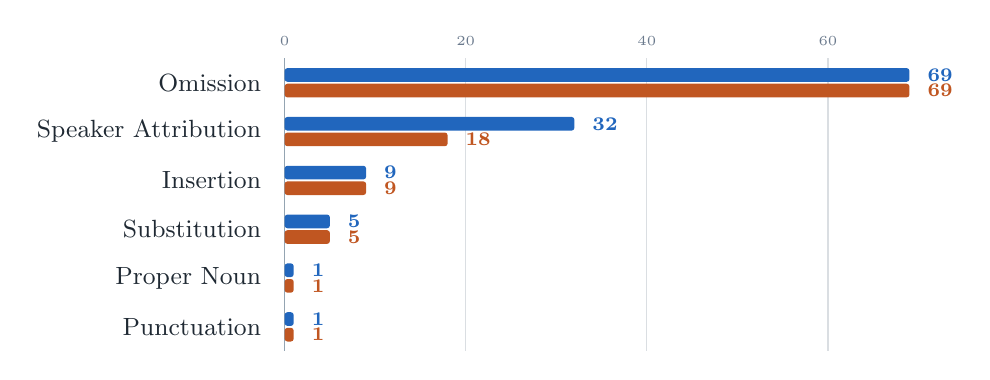
\begin{tikzpicture}[x=0.115cm, y=-0.62cm]
  \foreach \g in {0,20,40,60}{
    \draw[soft!25, line width=0.4pt] (\g,-0.5) -- (\g,5.5);
    \node[soft, font=\tiny, anchor=south, yshift=1pt] at (\g,-0.5) {\g};}
  \draw[hdr!55, line width=0.6pt] (0,-0.5) -- (0,5.5);

  \pairrow{0}{69}{69}{Omission}
  \pairrow{1}{32}{18}{Speaker Attribution}
  \pairrow{2}{9}{9}{Insertion}
  \pairrow{3}{5}{5}{Substitution}
  \pairrow{4}{1}{1}{Proper Noun}
  \pairrow{5}{1}{1}{Punctuation}
\end{tikzpicture}
\end{center}

\vspace{-0.2em}
{\footnotesize
\tikz[baseline=-0.55ex]\fill[barA, rounded corners=1pt] (0,0) rectangle (7pt,7pt);\,
\textcolor{soft}{large-v3 / wav2vec2 / pyannote}\qquad
\tikz[baseline=-0.55ex]\fill[warm, rounded corners=1pt] (0,0) rectangle (7pt,7pt);\,
\textcolor{soft}{large-v3 / wav2vec2 / Sortformer}}

\keybox{\textbf{Five bars cannot move and one can.} The typist is the same in both, so the
same words are right and wrong in both. Swapping \tagger{} changes exactly one bar --- and
that is the bar two thirds of Madison's sheet was about.}

\end{frame}

%----------------------------------------------------------
\begin{frame}{What the computed grade cannot say}

\begin{nicetable}{p{5.2cm}p{7.6cm}}
\hd{She recorded} & \hd{Why a program cannot} \\ \midrule
\textbf{Severity}, \textbf{Meaning Changed}
  & A judgement about the session, not a property of the text. Two identical word swaps can
    matter enormously and not at all \\
\textbf{One row per error}
  & She logged one row per thing she decided had happened. This logs one finding per
    contiguous difference, so adjacent slips may split or merge \\
\textbf{Anything in seconds}
  & The key's times are interpolated (slide 21). Timing needs a measured reference, which
    is the next job on the list \\
\end{nicetable}

\vspace{0.1em}
So the computed profile is the \emph{same kind} of number as hers, not the identical number.

\keybox{The check that \emph{is} free: grade the arm she actually read. The key is that arm
plus her 117 corrections, so her sheet and the computed profile describe the same errors ---
and a classifier that disagrees with her about what an omission \emph{is} shows up there,
before any other cell is believed.}

\end{frame}

%----------------------------------------------------------
\begin{frame}{Where this leaves us}

\begin{enumerate}
\itemsep 0.5em
\item A person listened for fifty minutes and logged \num{117} errors. \num{75} of them are
      about \emph{who spoke}, not about spelling.
\item Each row becomes one of four edits. \num{89} turns became \num{215}.
\item That transcript is the first thing here that can tell a model it is wrong --- and it
      already inverted the guess we would have used to name the speakers.
\item Three models to test, not one. The grid is a cube: \num{40} cells from \num{13} jobs.
\item And nobody listens again. Every cell is graded against her transcript in her own
      categories, which is \num{39} more listening passes we do not have to ask for.
\end{enumerate}

\bigidea{We built nothing on top of this transcript until somebody checked it.\\[3pt]
Now that it is checked, it is what checks everything else.}

\end{frame}

\end{document}
